\documentclass[a4paper,12pt]{report}

%\newcommand{\song}{\CJKfamily{song}}  %设置全局字体宋体 12pt = 小四
\usepackage{ctex}
\usepackage{xeCJK}    % CJK 包
\usepackage{times} %英文默认new Roman
\usepackage{setspace}
\usepackage{fancyhdr}
\usepackage{graphicx}
\usepackage{wrapfig}
\usepackage{array}  
\usepackage{fontspec,xunicode,xltxtra}
\usepackage{titlesec}
\usepackage{titletoc}
\usepackage[titletoc]{appendix}
\usepackage[top=30mm,bottom=30mm,left=20mm,right=20mm]{geometry}
\usepackage{cite}
\usepackage{listings}
\usepackage{float}
\usepackage[framed,numbered,autolinebreaks,useliterate]{mcode} % 插入代码
\XeTeXlinebreaklocale "zh"
\XeTeXlinebreakskip = 0pt plus 1pt minus 0.1pt

\setmainfont{Times New Roman}    % 设置西文字体

%---------------------------------------------------------------------
%	页眉页脚设置
%---------------------------------------------------------------------
\fancypagestyle{plain}{
	\pagestyle{fancy}      %改变章节首页页眉
}

\pagestyle{fancy}
\lhead{\kaishu~计算机系统报告~}
\rhead{\kaishu~1111111111 魏于翔~}
\cfoot{\thepage}

%---------------------------------------------------------------------
%	章节标题设置
%---------------------------------------------------------------------
\titleformat{\chapter}{\centering\zihao{-2}\heiti}{\heiti \thechapter}{1em}{} % 黑体小二号
\titlespacing{\chapter}{0pt}{*0}{*6}

\titleformat{\section}{\zihao{-3}\heiti}{\heiti \thesection}{1em}{} % 黑体小三号
%\titlespacing{\section}{0pt}{*0}{*6}

\titleformat{\subsection}{\zihao{4}\heiti}{\heiti \thesubsection}{1em}{} % 黑体四号

%---------------------------------------------------------------------
%	摘要标题设置
%---------------------------------------------------------------------
\renewcommand{\abstractname}{\centering\zihao{-2}\heiti 摘\quad 要}

%---------------------------------------------------------------------
%	参考文献设置
%---------------------------------------------------------------------
\renewcommand{\bibname}{\zihao{2}{\hspace{\fill}参\hspace{0.5em}考\hspace{0.5em}文\hspace{0.5em}献\hspace{\fill}}}

%---------------------------------------------------------------------
%	引用文献设置为上标
%---------------------------------------------------------------------
\makeatletter
\def\@cite#1#2{\textsuperscript{[{#1\if@tempswa , #2\fi}]}}
\makeatother

%---------------------------------------------------------------------
%	目录页设置
%---------------------------------------------------------------------
\titlecontents{chapter}[0em]{\heiti \zihao{-4}}{\heiti \thecontentslabel\ }{}
{\hspace{.5em}\titlerule*[4pt]{$\cdot$}\contentspage}
\titlecontents{section}[2em]{\vspace{0.1\baselineskip}\songti\zihao{-4}}{\thecontentslabel\ }{}
{\hspace{.5em}\titlerule*[4pt]{$\cdot$}\contentspage}
\titlecontents{subsection}[4em]{\vspace{0.1\baselineskip}\songti\zihao{-4}}{\thecontentslabel\ }{}
{\hspace{.5em}\titlerule*[4pt]{$\cdot$}\contentspage}


\begin{document}
%---------------------------------------------------------------------
%	封面设置
%---------------------------------------------------------------------
\begin{titlepage}
	\begin{center}
		
    
\includegraphics[width=0.6\textwidth]{figure//HIT.jpg}\\
    \vspace{1cm}
    \textsc{\LARGE Harbin Institute of Technology}\\[1.5cm]
    	
	% 标题
	\hrulefill \\[0.4cm]
	{ \huge \bfseries Y86指令集的SEQ模式CPU设计}\\[0.4cm]
	\hrulefill \\[1.5cm]
	
	\vspace{\fill}
	
\setlength{\extrarowheight}{3mm}

{\songti\zihao{3}	
\begin{tabular}{rl}
	
	%作者信息
	{\makebox[4\ccwd][s]{姓\qquad 名:}}& ~\kaishu 魏\quad 于\quad 翔\\
	
	{\makebox[4\ccwd][s]{学\qquad 号:}}& ~\kaishu 1111111111 \\ 

    {\makebox[4\ccwd][s]{学\qquad 院:}}& ~\kaishu 计算机科学与技术学院\\ 
   	
\end{tabular}
 }\\[2cm]
\vspace{\fill}

{\large \today}% 底部插入当日日期

	\end{center}	

\end{titlepage}


%---------------------------------------------------------------------
%  摘要页
%---------------------------------------------------------------------
\pagenumbering{Roman} %罗马数字

\chapter *{ 摘 {\quad} 要}
\setcounter{page}{1}
\addcontentsline{toc}{chapter}{\heiti 摘要}  %单独插入摘要 以章的形式
\begin{spacing}{1.5}
{\zihao{-4}
	此处为摘要
	
	此处为摘要\\[0.5cm]
	
	\textbf{ \heiti 关键字}:\quad 摘要 \quad 摘要 \quad 摘要 \quad 摘要
}。
\end{spacing}


\chapter *{ Abstract }
\addcontentsline{toc}{chapter}{\heiti Abstract}  %单独插入摘要 以章的形式 可选 part, section, subsection
\begin{spacing}{1.5}
	{\zihao{-4}
		此处为摘要
		
		此处为摘要\\[0.5cm]
		
		\textbf{ \heiti 关键字}:\quad 摘要 \quad 摘要 \quad 摘要 \quad 摘要
	}。
\end{spacing}

%---------------------------------------------------------------------
%  目录页
%---------------------------------------------------------------------
\tableofcontents % 生成目录


%---------------------------------------------------------------------
%  实验一
%---------------------------------------------------------------------

\chapter{Y86-64指令集体系结构}
\pagenumbering{arabic} %改为阿拉伯数字
\setcounter{page}{1}
\begin{spacing}{1.5} %行间距?
\songti\zihao{-4}
\section{基本变量}
	CPU中共有15个64位的程序寄存器,指示指令的PC的长度也为64位。CPU还有三个标志位,分别是零标志zf、符号标志sf、溢出标志of,这三个标志位统称为CC。
	
	我们要实现的CPU还增加了一条指令IADDQ,功能如下图1.3:
	
	\begin{figure}[htb]
		\centering
		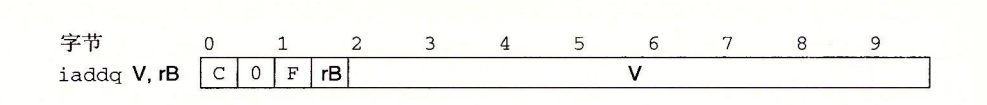
\includegraphics [width=1\textwidth]{figure/IADDQ.png}
		\caption{IADDQ指令}\label{Y86-64}
	\end{figure}

\section{指令编码}

	
\section{Y86-64异常}
	
\section{Y86-64程序}
	

\end{spacing}

%---------------------------------------------------------------------
%  实验二
%---------------------------------------------------------------------
\chapter{Y86-64的顺序实现}
\begin{spacing}{1.5}
\section{SEQ}
	SEQ处理器将指令的执行过程分为了六个过程,分别是取指(fetch)、译码(decode)、执行(execute)、访存(memory)、写会(wirte back)、更新PC(PC update)。同时CPU只有一个算数/逻辑单元,根据所执行的指令类型的不同,而进行不同的运算。
	
\section{指令微操作}
	
\section{SEQ硬件结构}

\section{SEQ的时序}

\end{spacing}


%---------------------------------------------------------------------
%  实验二
%---------------------------------------------------------------------
\chapter{SEQ阶段分析和HCL实现}
\begin{spacing}{1.5}
	
\section{取指阶段}	

\section{译码和写回阶段}
	
\section{执行阶段}
	

\section{访存阶段}
	
\section{更新PC阶段}
	
\end{spacing}

SEQ的全部实现代码见附录I。


%---------------------------------------------------------------------
%  实验二
%---------------------------------------------------------------------
\chapter{Verilog实现}
\begin{spacing}{1.5}
	
\section{实现过程}

\subsection{顶层模块设计}
	

\subsection{Fetch阶段设计}
	
\subsection{Decode阶段设计}
	分析3.2中的硬件结构可知,Decode阶段需要的输入有clk,rst,icode,ifun,rA,rB,输出有srcA,srcB。本阶段主要根据icode来确定srcA和srcB的值,最终从寄存器取值是在regfile模块进行的。
	\begin{lstlisting}
	module	Decode(
	input wire clk,
	input wire rst,
	input wire [3:0]icode,
	input wire [3:0]ifun,
	input wire [3:0]rA,
	input wire [3:0]rB,
	output reg [3:0]srcA,
	output reg [3:0]srcB
	);
	\end{lstlisting}
	

\subsection{Execute阶段设计}
	

\subsection{Memory阶段设计}
	

\subsection{Write back阶段实现}
	Write back阶段的硬件结构与译码阶段相同,但该阶段的工作是向寄存器中写入值,应有的输入有clk,rst,Cnd,icode,rA,rB,输出有dstM,dstE,该输出会作为regfile的控制逻辑。dstM和dstE是根据icode和Cnd的值从rA,rB中选择的。以IRRMOVQ为例:
	

\subsection{PC update阶段设计}
	
\subsection{regfile设计}
	
\subsection{inst\_rom设计}
	
	
\section{结果模拟}
	
\end{spacing}

%---------------------------------------------------------------------
%  总结
%---------------------------------------------------------------------
%\titleformat{\chapter}{\centering\zihao{-2}\heiti}{}{1em}{}
\addcontentsline{toc}{chapter}{结论}
\chapter *{结 {\quad} 论}
\begin{spacing}{1.5}
	
\end{spacing}

%---------------------------------------------------------------------
%  参考文献设置
%---------------------------------------------------------------------
\addcontentsline{toc}{chapter}{参考文献}

\begin{thebibliography}{99}
\songti \zihao{-4} 	
	\bibitem{Leslie.{1994}}
	Leslie Lamport. LATEX: A Document Preparation System.AddisonWesley, Reading, Massachusetts, second edition, 1994, ISBN 0-201-52983-1.
	
	\bibitem{Donald.{1984}}
	Donald E. Knuth. The TEXbook, Volume A of Computers and Typesetting,Addison Wesley, Reading, Massachusetts, second edition, 1984,ISBN 0-201-13448-9.Q

	
\end{thebibliography}

%---------------------------------------------------------------------
%  附录设置
%---------------------------------------------------------------------
\titleformat{\chapter}{\heiti\Large}{附录~\Alph{chapter}}{11pt}{\Large}
\titlespacing{\chapter}{0pt}{*-4}{*4}
\lstset{breaklines}                %自动将长的代码行换行排版
\lstset{extendedchars=false}
\lstset{language=Matlab}
\renewcommand{\thechapter}{附录\Alph{chapter}.} 
\appendix
\begin{appendix}
	
\chapter{数据表}
\zihao{-4}\songti
\begin{spacing}{1.5}
	hello world!
\end{spacing}


\chapter{程序代码}
\zihao{-4}\songti
\begin{spacing}{1.5}
下面是一个MATLAB程序的事例,使用了Package mcode,它能较好还原MATLAB本身的编写风格。
\begin{lstlisting}

\begin{lstlisting}
	module Write(
	input wire clk,
	input wire rst,
	input wire Cnd,
	input wire [3:0] icode,
	input wire [3:0] rA,
	input wire [3:0] rB,
	output reg [3:0] dstM,
	output reg [3:0] dstE
	);
	\end{lstlisting}
	
	\begin{lstlisting}
	`IRRMOVQ:	begin  // 也是CMOV
		dstE = Cnd == 1 ? rB : `RNONE;
		dstM = `RNONE;
	end
\end{lstlisting}

\end{lstlisting}
\end{spacing}
\end{appendix}

	

\end{document}
